\chapter{Problema de Investigación y Definición del Problema}
\section{Introducción}

    Hoy en día, dada una gran cantidad de usuarios concurrentes o un gran flujo de eventos que generan entradas, el software debe desarrollarse con una arquitectura y sobre una infraestructura capaz de soportar semejantes cargas de trabajo. Ante estas condiciones, una alternativa es el desarrollo de aplicaciones con una Arquitectura Orientada a Servicios y con tecnologías de virtualización, todo esto con el objetivo de hacer uso eficiente de los recursos y procesos y, por lo tanto, costos.
    
    Por otro lado, el estado del arte de la electrónica ha facilitado una variedad de herramientas capaces de mejorar los procesos industriales, los sistemas en general y, además, proporcionar una mayor calidad de vida a la sociedad. Al hacer uso de las herramientas que proporciona la electrónica y de la creatividad de las soluciones de software, las aplicaciones alcanzan armonía con los objetivos de optimización y reducción de costos de las empresas y ciudades. 
    
    En 2015, más de 72.37 millones de vehículos fueron vendidos en el mundo \cite{Statista2016-qw} y según la \citeA{Interpol2015-lz}, hubieron más de 7.4 millones de reportes de vehículos robados mundialmente. Cuando se habla de hacer un seguimiento de los vehículos, esfuerzo humano innecesario es requerido y las compañías incurren en costos que preferirían evitar.
    
    En este sentido, dado el nivel de la tecnología en el área de la visión artificial, unido con útiles herramientas que proporciona la electrónica, los sistemas de seguridad no sólo sirven para proteger bienes e inmuebles, sino también personas , además de ahorrar tiempo y dinero. Por ejemplo, países como Estados Unidos cuentan con sistemas de reconocimiento de matrículas en la ciudad para el seguimiento de infracciones \cite{ACLU2016}. 
    
    Cabe recalcar que el manejo de la información en cualquier tipo de institución es crucial para la toma de decisiones. Por ello, el acceso a la misma debe ser rápido y eficiente. En Santa Cruz de la Sierra, se ha identificado la necesidad de desarrollar una aplicación que sea capaz de reconocer que vehículos acceden o salen de una empresa, urbanización o estacionamiento, y, además, sea capaz de soportar las cargas de procesamiento que requiera este proceso, haciendo un uso eficiente de los recursos tanto humanos como de computación para reducir costos e incrementar la seguridad de las empresas.
\section{Definición del Problema}
Previa recopilación de datos se pudo recolectar información acerca de las falencias en cuanto a la utilización de sistemas de seguridad para el control vehicular. Las falencias encontradas son las siguientes:
\begin{itemize}
  \item En un contexto local, no se utilizan tecnologias de la nube para el desarrollo de servicios o aplicaciones en la nube (privada o pública), ni se promueve el desarrollo utilizando Arquitecturas Orientadas a Servicios, lo cual es una deficiencia pues no se considera ni refuerza la interoperabilidad, reusabilidad/bajo acoplamiento, aislamiento de errores, aprovechamiento de recursos tanto virtuales como físicos, etc.. 
  \item Las instituciones locales no suelen contar con soluciones que proporcionen descriptores visuales para el manejo de la información registrada en los vídeos de las cámaras de seguridad. 
  \item No existen soluciones que identifiquen matriculas o cumplan con la tarea del punto anterior a bajo costo y adaptadas al mercado local que aporten a la seguridad de las instituciones.
  \item También se tiene deficiencias en cuanto a la recopilación de información correspondiente a los vehículos que ingresan a la institución, generación de reportes y monitoreo de los vehículos.
\end{itemize}

    \subsection{Situación Problemática}
    Las soluciones que permitan obtener información de los vehículos identificados requieren de inversiones altas que prefieren ser evitadas. Dado lo anterior, se opta por utilizar recursos humanos para mantener registros físicos, lo cual requiere costos de personal, además de tiempo y esfuerzo que puede ser utilizado en otras tareas de mayor nivel.
    
    En caso de necesitar hacer una consulta para encontrar un vehículo, se debe recorrer secuencialmente todo el vídeo en los registros de vídeo de las cámaras de seguridad, lo cual es ineficiente dado el estado del arte de las tecnologías de visión artificial.
    \subsection{Situación Deseada}
    Automatizar el proceso de reconocer matrículas y el de proveer información sobre las matriculas identificadas y sus respectivos propietarios, facilitar los reportes sobre el monitoreo de las matrículas y notificar si se observa una matrícula sospechosa.
    \subsection{Objeto de Estudio}
        \begin{figure}[H]
            \centering
            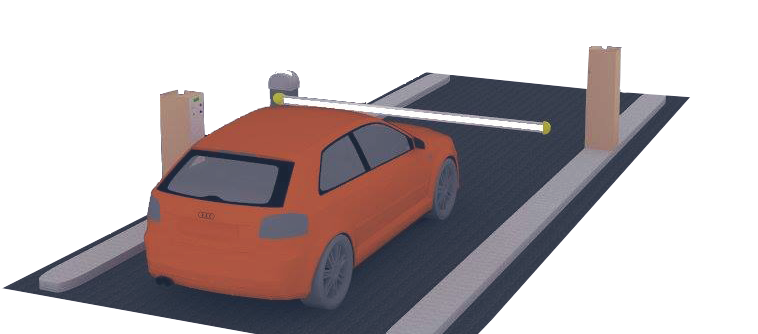
\includegraphics[width=\textwidth]{auto}
            \caption{Ingreso de vehículos a un parqueo}
            % \caption{Distribución del software en nodos y su integración con cámaras de seguridad}
            \label{fig:auto}
        \end{figure}
        El objeto de estudio, representado en la figura \ref{fig:auto}, en el PFG es el proceso de identificación de matriculas cuando se observa un vehículo, y el desarrollo de una aplicación orientada a servicios (SOA).

\section{Objetivos}

    \subsection{Objetivo General}
    Desarrollar un prototipo de Aplicación Nativa de la Nube con Reconocimiento Automático de Matriculas para el Control Vehicular para la empresa QSS Bolivia, y utilizando Kubernetes y las librerías open-source de visión artificial OpenCV  y OpenALPR, aplicable a un contexto operacional realista.
    \subsection{Objetivos Específicos}
    \begin{itemize}
    \item Identificar y recolectar los requerimientos y/o requisitos con el fin de obtener toda la información necesaria para el análisis y elaboración del Software.
    \item Realizar reuniones con los encargados de la empresa a fin de recabar más información de las cámaras que se usan en las instalaciones, la ubicación de las mismas y sus especificaciones.
    \item Analizar y evaluar los requerimientos funcionales y no funcionales.
    \item Diseñar y modelar los diferentes artefactos de software tomando como base el análisis de requisitos utilizando una metodología de desarrollo de software ágil.
    \item Diseñar e implementar una base de datos capaz de soportar todos los requerimientos del software.
    \item Utilizar algoritmos de visión artificial para realizar el reconocimiento de matriculas.
    \item Implementar la conexión a la cámara de seguridad.
    \item Implementar la detección y la traducción de una matrícula en el momento del ingreso o salida (en tiempo real) de una manera óptima.
    \item Ajustar el post-procesamiento de comparación de los posibles dígitos de matrículas reconocidos para que este acorde con la plantilla de matrícula boliviana.
    \item Realizar pruebas necesarias para garantizar que el software desarrollado cumpla con los requerimientos del cliente.
    \item Evaluar las distintas tecnologías de administración de contenedores para aplicaciones nativas de la nube. 
    \item Representar visualmente la diferencia del diseño de la aplicación monolítica a una aplicación orientada a servicios.
    

    \end{itemize}
\section{Metodologia}
\subsection{Contexto de Ágil}
En el momento de definir la metodología más adecuada para el Proyecto Final de Grado (PFG) es esencial tomar en cuenta la naturaleza del mismo.

El PFG aprovecha las ventajas de la computación en la nube de acuerdo con los lineamientos establecidos en el Capítulo II y hace uso tecnologías de visión artificial para el procesamiento de imágenes digitales (Capítulo III-IV). 

    \begin{figure}[H]
        \centering
        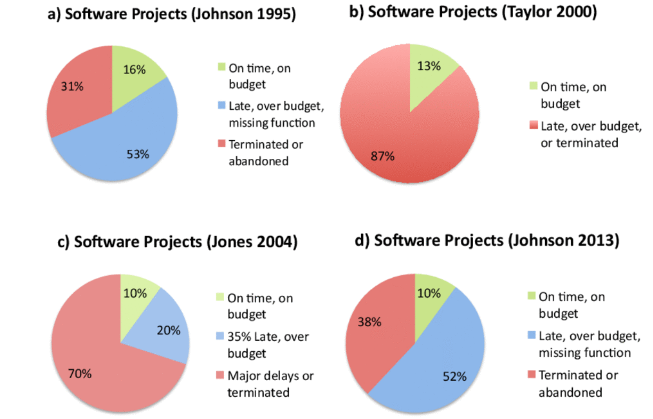
\includegraphics[width=1\textwidth]{pp-sw-projects}
        \caption{Figura de encuestas \protect\cite{Fox2013-ct}}
        \label{fig:pp-sw-projects}
    \end{figure}

Como se observa en la Figura \ref{fig:pp-sw-projects}, \citeA{Johnson1995-yr}, \citeA{Taylor2000-yr}, \citeA{Jones2004-vq} y \citeA{Johnson2013-yr} reflejan la crisis del software que no llega a poder ser entregado dentro del tiempo ni presupuesto establecidos. 

Dado esto, surge la necesidad de una metodología de software que pueda lidiar con los cambios que ocurren en los proyectos de software de manera continua y con una mayor interacción con el cliente. \citeA{Johnson2013-yr} demuestra que los proyectos pequeños, que típicamente utilizan metodologías ágiles, tienen mayor probabilidad de ser exitosos que proyectos grandes (76\% de los proyectos se terminan a tiempo y sobre el presupuesto). 
    
    \begin{figure}[H]
            \centering
            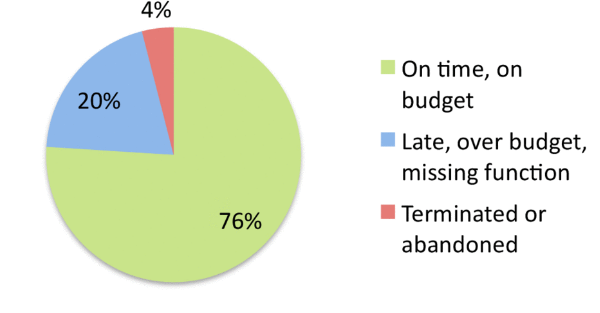
\includegraphics[width=0.90\textwidth]{pp-sw-small}
            \caption{Figura de encuestas \protect\cite{Fox2013-ct}}
            \label{fig:pp-sw-small}
        \end{figure}

En este sentido, se alcanza una armonía entre la naturaleza SaaS del PFG y las características de las metodologías ágiles, al estar el PFG  bajo una perspectiva de descomposición en componentes con interfaces bien definidas (Capítulos II y VI), la constante interaccion con el cliente y entrega de prototipos.

\subsection{ICONIX}
Dado el contexto de ágil, descrito en la sección anterior y la experiencia en proyectos pasados utilizando el Proceso Unificado de Rational (RUP), se definió que la metodología ágil más adecuada para el PFG es ICONIX, basado en lo que establecen \citeA{Rosen05-ct}, en \textit{Agile Development with ICONIX Process: People, Process, and Pragmatism}. 

ICONIX mantiene las características esenciales de RUP sin discriminar la importancia de la documentación del software; la cual ICONIX considera es esencial independiente de la complejidad del proyecto. 
Mas aún, ICONIX establece un enlace crucial entre el análisis y el diseño, solventando la grieta que existe entre ambos. Esto lo hace con sus estereotipos de análisis (objetos de frontera, control y entidad), los cuales se traducen con relativa sencillez a Arquitecturas MVC \cite{Rosen05-ct}; este es otro de los beneficios que ICONIX trae para el PFG. Las arquitecturas MVC se describen brevemente en la sección de patrones de Arquitecturas SaaS en el Capitulo VI. 
En ICONIX, los artefactos requeridos son:
\begin{itemize}
  \item Texto de Casos de Uso: definir los requerimientos de comportamiento.
  \item Modelo de Dominio: describir los objetos del mundo real y sus relaciones.
  \item Diagrama de Robustez: Disminución de los requerimientos de comportamiento.
  \item Diagrama de Secuencia: Asignar comportamiento a las clases.
  
\end{itemize}

\begin{figure}[H]
            \centering
            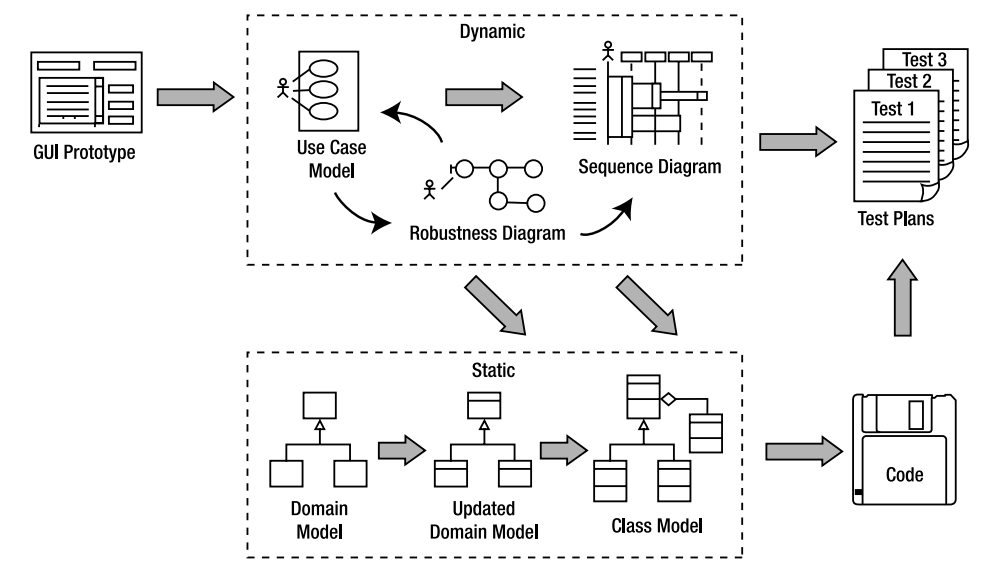
\includegraphics[width=\textwidth]{iconix-process}
            \caption{Proceso ICONIX \protect\cite{Rosen05-ct}}
            \label{fig:iconix-process}
        \end{figure}

En pocas palabras, para cada escenario y complementando con la Figura \ref{fig:iconix-process}, el proceso ICONIX puede descomponerse en:
\begin{enumerate}
    \item Identificar los objetos de dominio del mundo real (modelado del dominio)
    \item Definir los requerimientos de comportamiento (casos de uso)
    \item Realizar el análisis de robustez
    \item Asignar comportamiento a los objetos (diagrama de secuencia)
    \item Finalizar el modelo estático (diagrama de clases)
    \item Implementar el escenario
    \item Realizar pruebas
\end{enumerate}

Donde los hitos que se deben alcanzar en cada entregable son:
\begin{enumerate}
    \item Revisión de Requerimientos
    \item Revisión Preliminar del Diseño
    \item Revisión Detallada/Critica del Diseño
    \item Entrega
\end{enumerate}